\mainmatter
\setcounter{page}{1}

\lectureseries[\course]{\course}

\auth[\lecAuth]{Lecturer: \lecAuth\\ Scribe: \scribe}
\date{August 1, 2015}

\setaddress

% The following hack starts the lecture numbering at 1.
\setcounter{lecture}{0}
\setcounter{chapter}{0}

\lecture{Physics Final Review}

\section{Periodic Motion}
Periodic motion is motion that repeats over and over again, also known as oscillations. A body that undergoes periodic motion always has a stable equilibrium position. 

\subsection{Describing Oscillations}
The simplest way to define the origin of the system is at the equilibrium position. When a system is displaced form equilibrium, there is always a restoring force to put the system back into equilibrium position. The restoring force pulls the body 
 

$\vdots$

\subsection{Definitions}

The \textit{amplitude} of the motion ($A$) is the maximum magnitude of displacement from equilibrium.

$\vdots$

These values are related via the following equations.

\begin{align}
\label{eq:freq}
f = \frac{1}{T} 
\end{align}

Frequency is defined in Equation \ref{eq:freq}.

\begin{figure}[ht!]
	\centering
	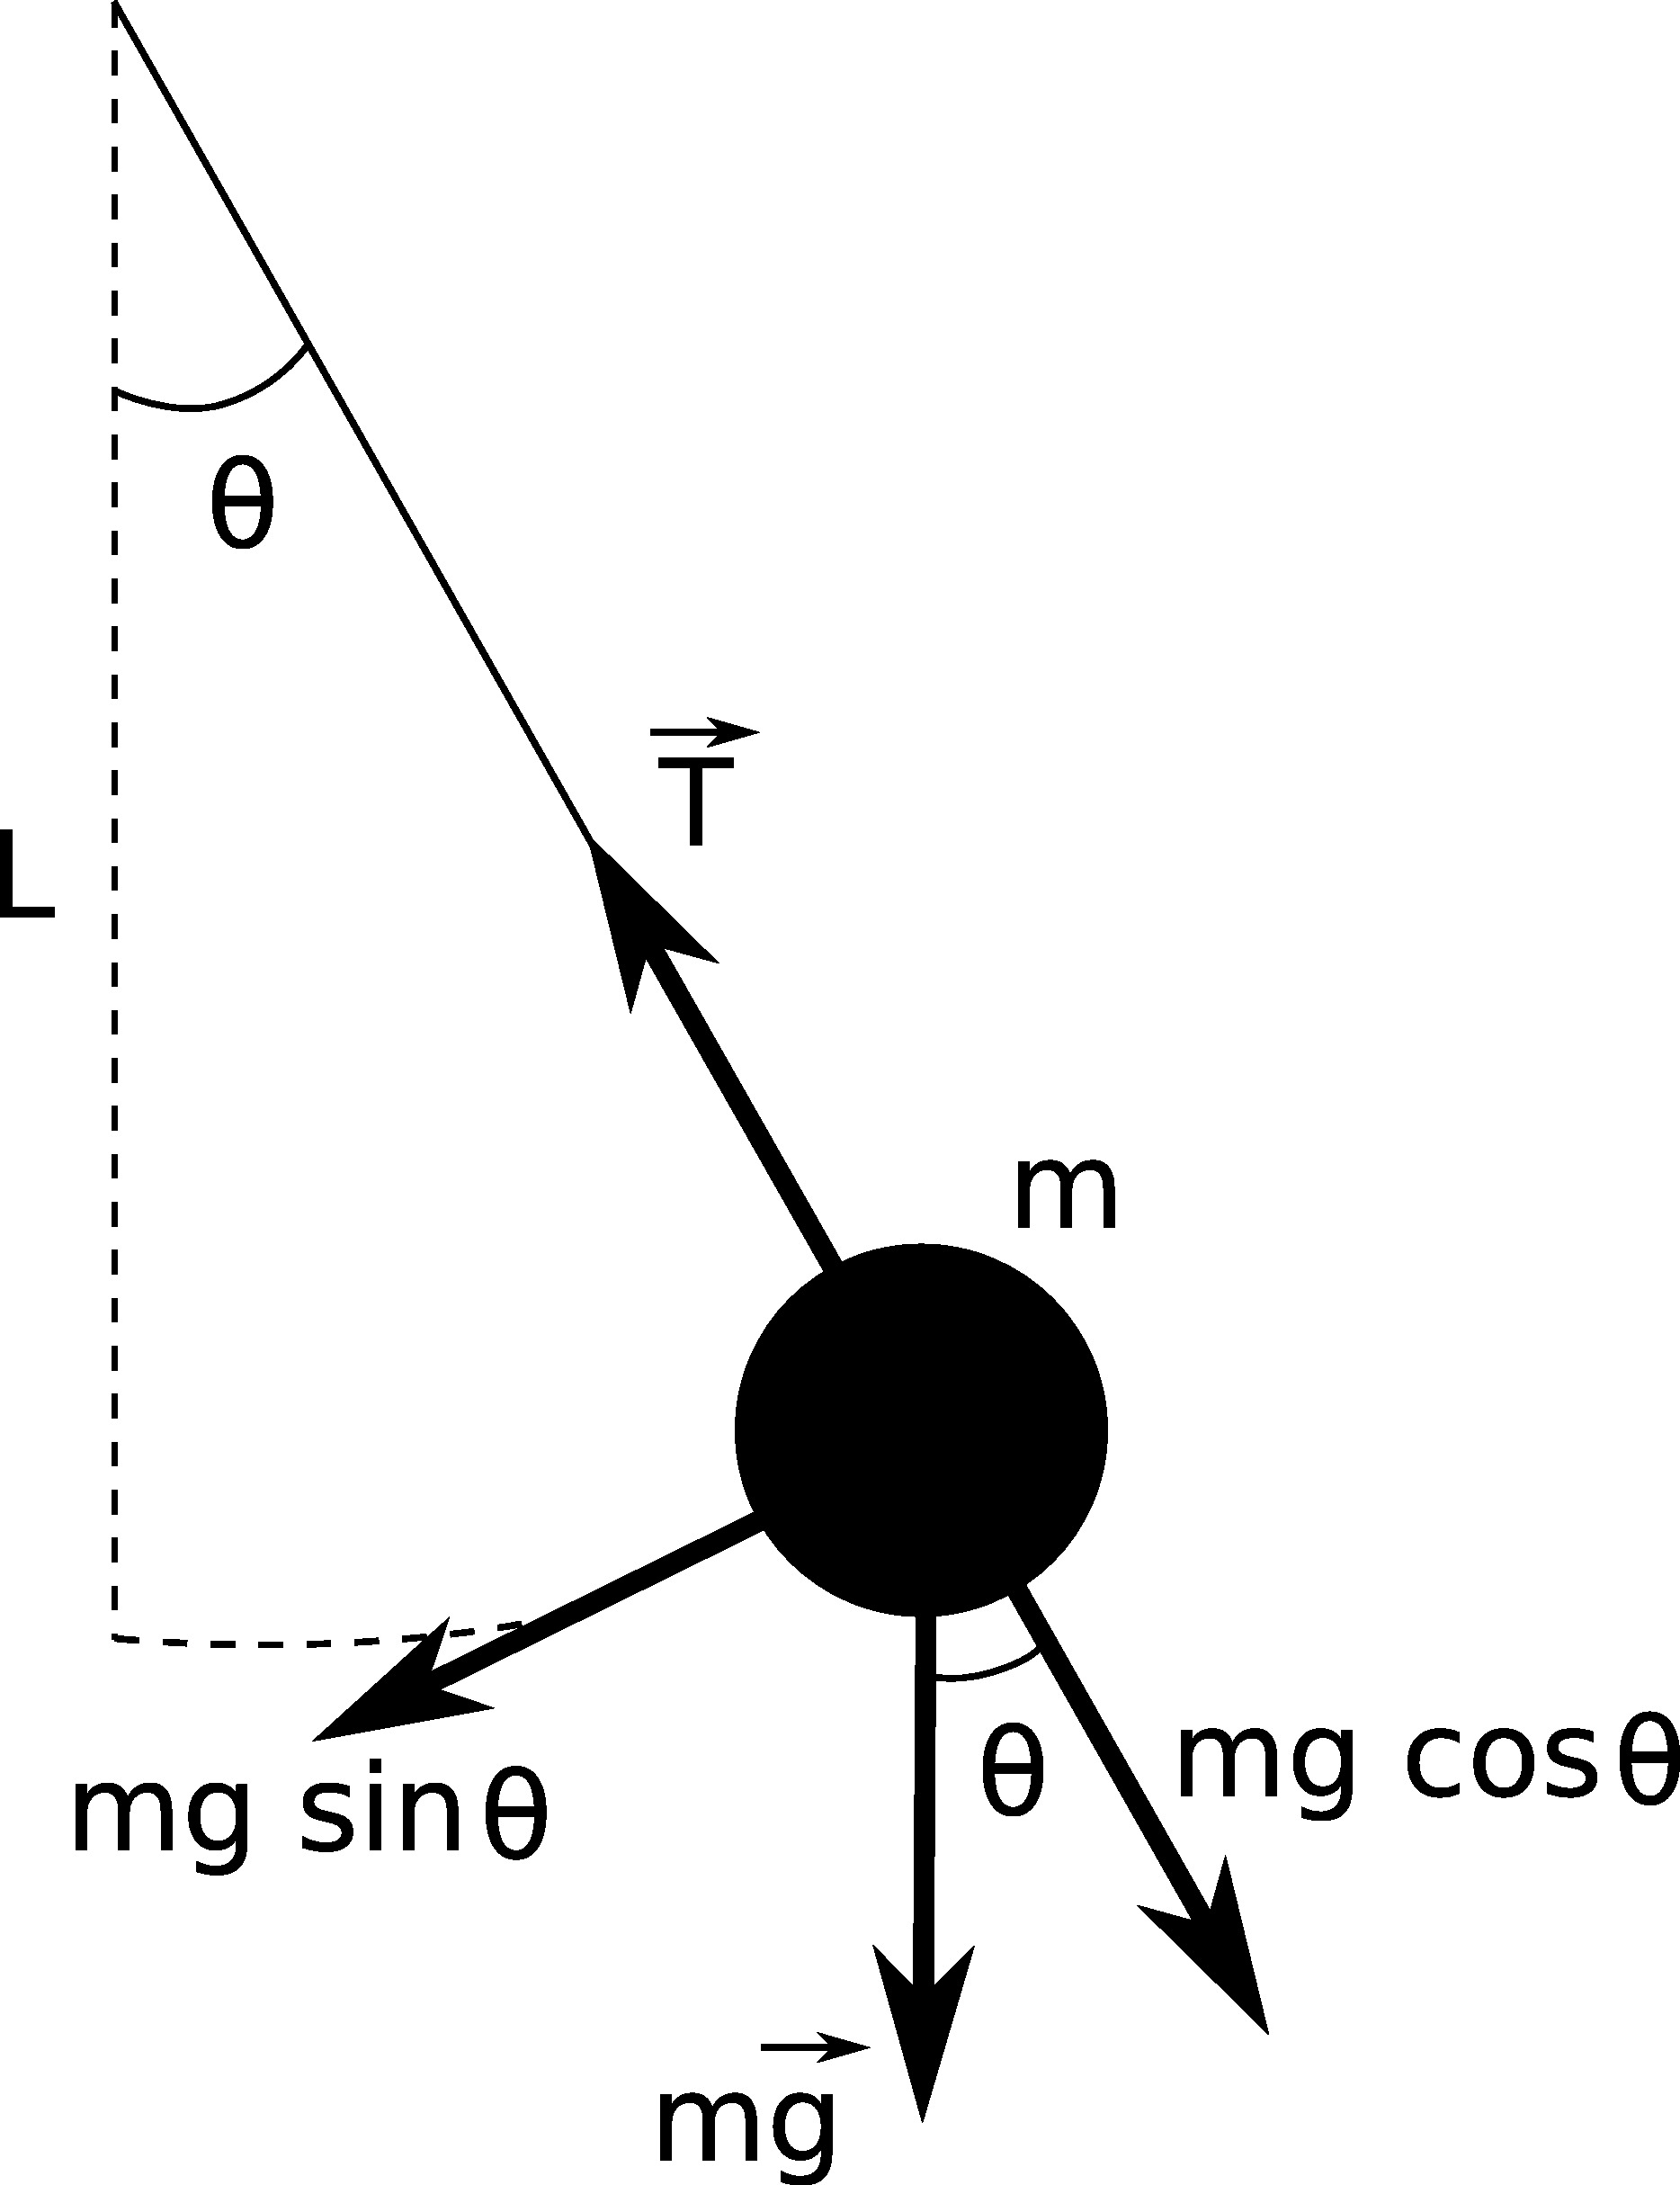
\includegraphics[width=.6\textwidth]{images/01pendulum}
	\caption{Pendulum.}
	\label{fig:01pendulum}
\end{figure}

Figure \ref{fig:01pendulum} shows a pendulum. Note: inkscape

\section{Course Notes}
Course notes.
